
\section{Workflow Of A Metabolomics Experiment}

Regarding metabolomics, there are four conceptual approaches: target analysis, metabolite profiling,  metabolomics, and metabolic fingerprinting \citep{roessner2009metabolomics}. The general workflow of the various metabolomics approaches is shown in \autoref{workflow}. Target analysis includes the determination and quantification of a small set of known metabolites, also called targets, making use of one particular analytical technique that shows the best performance for the compounds of interest. It has been applied for many years, including, for instance, in the analysis of head and neck cancer cells \citep{hu2015targeted}.

Metabolite profiling is different than the previous approach in the sense that it aims at the analysis of a larger set of compounds. Regarding their chemical structure, these compounds are both identified and unknown and their quantification either quantitative or semi-quantitative (an absolute quantification is not required). This approach is widely applied and has been used for instance in the identification of kidney cancer using urine's metabolic signatures \citep{kind2007comprehensive}.

The metabolomics approach employs complementary analytical methodologies, including \gls{lcms}, \gls{gcms} and/or \gls{nmr} techniques, to determine and quantify as many metabolites as possible. Similarly to the previous approach, the compounds can be either identified or unknown. It is widely used, having been applied in the determination of natural stress influence on the metabolic status of sea snail \citep{rosenblum2005characterizing}.

Lastly, in a metabolic fingerprinting approach, a metabolic "signature" or mass profile of the sample of interest is generated and then compared in a large sample population to screen for differences between the samples, it is most typically used for sample classification based on its spectrum. If the metabolites to analyze are either external and/or secreted by the cells then it is called footprinting approach. If signals that can significantly discriminate between samples are detected, then the metabolites can be identified and the biological relevance of that compound elucidated, saving valuable analysis time. It is commonly used in forensics, among other fields, having been applied for instance in the discrimination of blue ball-point pen inks \citep{thanasoulias2003multivariate}. This approach will be emphasized throughout this dissertation.

The main steps in a metabolic fingerprinting experiment are: sample preparation, data acquisition, pre-processing, data analysis and data interpretation. Upon sample preparation and data acquisition the data is then preprocessed to allow an improved analysis, where the objective is to extract useful knowledge from the data. The pre-processing and analysis steps will be the main focus throughout this dissertation.

\begin{figure}[!ht]
	\centering
	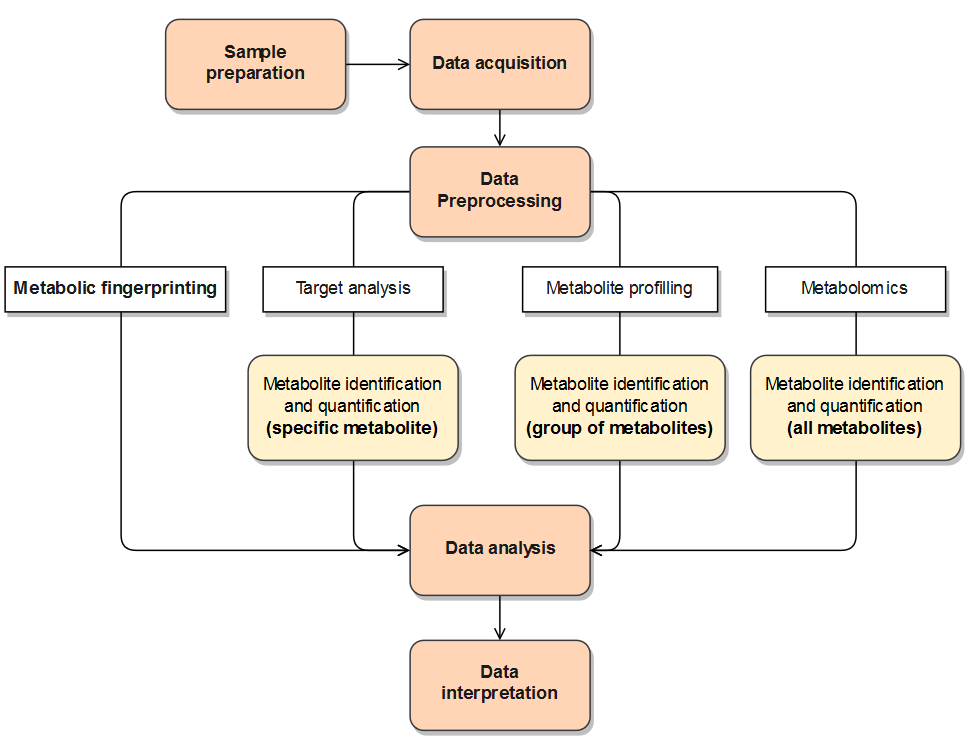
\includegraphics[width=0.9\linewidth]{Imagens/workflow}
	\caption{General workflow of the various metabolomics approaches.}
	\label{workflow}
\end{figure}


\subsection{Preprocessing}

The pre-processing step covers all editing of the data up to the point of starting the analysis. This is a crucial step in any metabolomics experiment, making samples analyzable and comparable. In a metabolic fingerprinting approach, the most commonly used pre-processing methods include missing values and outlier removal, normalization or scaling, derivative calculation, mean centering and some peak spectra processing. The order in which the pre-processing steps are applied to the data is not always obvious, being sometimes governed more by practical considerations than optimal statistical analysis. The methods discussed in this section are the ones most commonly used regarding \gls{ir}, \gls{uv} and Raman spectroscopies, the techniques focused on this dissertation.

When handling missing values, there are two main approaches: their removal or replacement. In the first approach, the value can be removed by either removing the feature or the sample containing it. In the latter, the value can be replaced using various methods, including its replacement by the row or column mean, or even using more sophisticated methods (e.g. nearest neighbors, linear approximation). Frequently, there are values within the dataset that are distant from all other observations, thus considered outliers. These are typically excluded from the dataset, as they could interfere in the subsequent analysis results.

Peak spectra pre-processing aims to perform corrections over the spectra. It includes for instance baseline and background correction and smoothing methods, among others. Baseline correction method is used to correct unwanted linear or non-linear additions to the spectra. These additions are often associated with equipment used when measuring samples (e.g. non-linearities in detectors) or, for instance, by the interference of a complex matrix. Depending on the situation, this method might be essential, considering most statistical analysis techniques cannot distinguish between baselines and signal. 

Background correction, as the name suggests, is applied to remove the background in the spectra. This background can be caused by various factors, including absorption associated with the sample holder and/or solvent used. 

The smoothing methods are used to filter spectra noise, and might be specially helpful when signal-to-noise ratio is high or the subsequent analysis methods are very sensitive to noise. It helps in both visual interpretation and robustness of the analysis, but it is important to balance noise reduction and peak retention, specially in the small peaks \citep{liland2011multivariate}. The Savitzky-Golay filter is one of the most popular smoothing methods. This method fits successive sub-sets of adjacent data points with a low-degree polynomial by the method of linear least squares, using a process known as convolution \citep{savitzky1964smoothing}.

Other commonly used peak spectra pre-processing methods include peak alignment and binning. In its simplest form, peak alignment consists in dividing the spectra in a number of local windows, where peaks are shifted to match across spectra. Since everything is done locally, peak alignment is a fast method, however, it may lead to misalignment when peaks fall into the wrong local window or are split into two windows. When continuous spectra are recorded producing tens or hundreds of thousands of measurements per spectrum, the binning method can be helpful. In this method, the spectrum is divided into a desired number of bins and all measurements inside each bin summed, forming new spectra with fewer variables. The simplest reason for binning is that the number of variables can be too high for handling of the problem in ordinary computer memory. There are, however, a few dangers regarding the bad placing of the bins, by removing information or producing false information \citep{liland2011multivariate}.

In many analytical methods, the variables measured for a given sample are subject to overall scaling or gain effects. Standardization methods attempt to correct for these kinds of effects by identifying some aspect of each sample which should be essentially constant between samples, giving all them an equal impact on the model. In the \acrfull{snv} method, a weighted normalization is performed (not all points contribute to the normalization equally). Therefore, the values are subtracted of their mean and then the result is divided by the standard deviation. Spectra treated in this manner have always zero mean value and a variance equal to one and are thus independent of original absorbance values. 

The \acrfull{msc} method is a relatively simple processing step that attempts to account for additive and/or multiplicative effects in spectral data. It does so by estimating light scattering or change in path length for each sample relatively to that of an ideal sample. Another method consists in centering the data, by calculating the average spectrum of the dataset and subtracting that average from each spectrum. In this method, the values are changed, but not the scale.

Derivative spectroscopy uses first or higher derivatives of absorbance with respect to wavelength for qualitative analysis and for quantification. Generally speaking, by differentiation of a zero order spectrum and obtaining consecutive derivative spectra the separation of overlapping peaks is achieved, increasing selectivity without separation of the analytes. First and second-order derivatives are the ones most commonly calculated. A graphical representation of first and second order derivatives calculation is shown in \autoref{derivatives}. The first-order derivative consists in the rate of change of absorbance with respect to wavelength, while the second-order derivative has a very characteristic feature consisting in a negative band with minimum at the same wavelength as the maximum on the original spectrum. This method can be useful because spectra that are very similar in absorbance mode may reveal significant differences in the derivative mode. Another advantage resides in the fact that because the first derivative of a constant absorbance offset is zero, calculating the first derivative spectra always eliminates baseline shifts \citep{kus1996derivative}.

\begin{figure}[!htb]
	\centering
	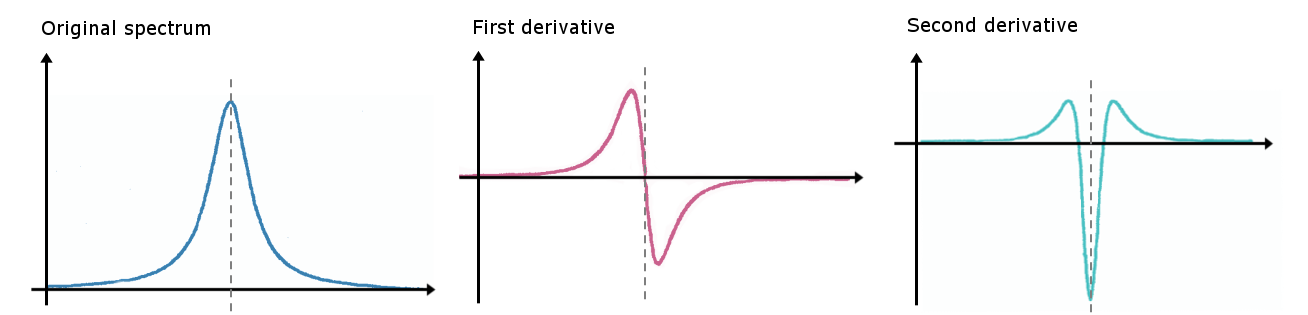
\includegraphics[width=1\linewidth]{Imagens/derivatives}
	\caption{Graphical representation of first and second order derivatives calculation.}
	\label{derivatives}
\end{figure}


The pre-processing methods applied can vary greatly between datasets and type of spectroscopy used. \textbf{\autoref{spectroscopies}} summarizes the various pre-processing methods used in several experiments from the literature (in the fourth column). In \gls{ir} spectroscopy, peak spectra processing methods are often applied, including smoothing and baseline correction. Normalization and scaling methods, including mean centering and \gls{snv} are also often used, as well as first and second-order derivatives calculation. Unlike \gls{ir} spectroscopy, in \gls{uv} experiments less pre-processing methods are applied, being normalization and first derivative calculation the most commonly applied methods. In Raman spectroscopy, the pre-processing methods usually applied are similar to those applied in \gls{ir} spectroscopy.





